\chapter{Experimental Evaluation}
\label{ch:evaluation}

\section{Dataset: Adult Census Income}

The Adult Census Income dataset~\cite{adultdataset} (also known as the ``Census Income'' dataset) contains 32,561 records extracted from the 1994 U.S.\ Census Bureau database. The prediction task is binary classification: whether an individual's annual income exceeds \$50,000. The dataset contains 14 features and exhibits significant class imbalance, with 17,303 instances (53.2\%) in the low-income class and 5,489 instances (16.9\%) in the high-income class.

Four protected attributes were selected for analysis: \textbf{age} (71 unique values), \textbf{race} (5 unique values), \textbf{sex} (2 unique values), and \textbf{native-country} (42 unique values).

\begin{table}[H]
\centering
\caption{Dataset split and model configuration.}
\label{tab:dataset}
\begin{tabular}{@{}lr@{}}
\toprule
\textbf{Parameter} & \textbf{Value} \\
\midrule
Total instances & 32,561 \\
Training set & 22,792 (70\%) \\
Validation set & 3,256 (10\%) \\
Test set & 6,513 (20\%) \\
Number of features & 14 \\
Hidden layers & $\langle 64, 32, 16, 8, 4 \rangle$ \\
Output neurons & 2 (binary) \\
Total parameters & 3,998 \\
Epochs trained & 30 \\
\bottomrule
\end{tabular}
\end{table}

\section{Model Training Results}

The proxy model achieved 85.34\% test accuracy, with final training loss of 0.356 and validation loss of 0.324. The gap where test accuracy exceeds training accuracy (85.34\% vs.\ 83.32\%) is attributable to early stopping restoring the best validation-loss model state, combined with Dropout being disabled during evaluation.

\begin{figure}[H]
    \centering
    \fbox{\parbox{0.85\textwidth}{\centering\vspace{0.5cm}
    \textbf{[INSERT FIGURE: Training History Plot]}\\[0.3cm]
    \textit{Plot showing training loss/accuracy and validation loss/accuracy over 30 epochs, demonstrating convergence and the early stopping behavior.}
    \vspace{0.5cm}}}
    \caption{Training and validation curves over 30 epochs.}
    \label{fig:training}
\end{figure}

\section{QID Analysis Results}

Analysis of 500 randomly sampled test instances reveals pervasive individual discrimination:

\begin{table}[H]
\centering
\caption{QID analysis results on the Adult Census dataset.}
\label{tab:qid}
\begin{tabular}{@{}lr@{}}
\toprule
\textbf{Metric} & \textbf{Value} \\
\midrule
Instances analyzed & 500 \\
Mean QID (Shannon entropy) & 0.640 bits \\
Max QID & 1.000 bits \\
Standard deviation QID & 0.311 bits \\
Mean min-entropy QID & 0.214 bits \\
Mean disparate impact ratio & 0.581 \\
Discriminatory instances (QID $> 0.1$) & 479 (95.8\%) \\
Instances violating 80\% rule & 349 (69.8\%) \\
\bottomrule
\end{tabular}
\end{table}

A mean QID of 0.640 bits out of a theoretical maximum of 1.0 bit for binary classification indicates that protected attributes carry substantial influence over predictions. The near-universal discrimination rate of 95.8\% demonstrates that the model changes its prediction for nearly every individual when protected attributes are altered. The mean disparate impact ratio of 0.581 falls well below the 0.8 legal threshold.

\begin{figure}[H]
    \centering
    \fbox{\parbox{0.85\textwidth}{\centering\vspace{0.5cm}
    \textbf{[INSERT FIGURE: QID Distribution Histogram]}\\[0.3cm]
    \textit{Histogram showing the distribution of QID values across 500 analyzed instances, with the 0.1-bit threshold line and the concentration of values near the maximum.}
    \vspace{0.5cm}}}
    \caption{Distribution of QID values across 500 analyzed instances.}
    \label{fig:qid_dist}
\end{figure}

\section{Group Fairness Results}

Table~\ref{tab:group_fairness} presents the group fairness metrics across all four protected attributes.

\begin{table}[H]
\centering
\caption{Group fairness metrics by protected attribute.}
\label{tab:group_fairness}
\small
\begin{tabular}{@{}l c c c c c@{}}
\toprule
\textbf{Attribute} & \textbf{DP Diff} & \textbf{DP Ratio} & \textbf{TPR Diff} & \textbf{FPR Diff} & \textbf{EO Max} \\
\midrule
Sex & 0.162 & 0.298 & 0.088 & 0.065 & 0.088 \\
Age & 0.181 & 0.344 & 0.097 & 0.078 & 0.097 \\
Race & 0.083 & 0.564 & 0.086 & 0.025 & 0.086 \\
Native-country & 0.042 & 0.769 & 0.021 & 0.012 & 0.021 \\
\bottomrule
\end{tabular}
\end{table}

The \textbf{sex} attribute exhibits the most severe bias: a demographic parity ratio of 0.298 (far below the 0.8 threshold) indicates that Group~A (female, $n=2{,}158$) receives positive predictions at only 6.9\% compared to 23.1\% for Group~B (male, $n=4{,}355$). The \textbf{age} attribute shows similarly concerning disparities with a DP ratio of 0.344. The \textbf{race} attribute has moderate bias (DP ratio 0.564), while \textbf{native-country} shows the least disparity (DP ratio 0.769, approaching fairness).

\begin{figure}[H]
    \centering
    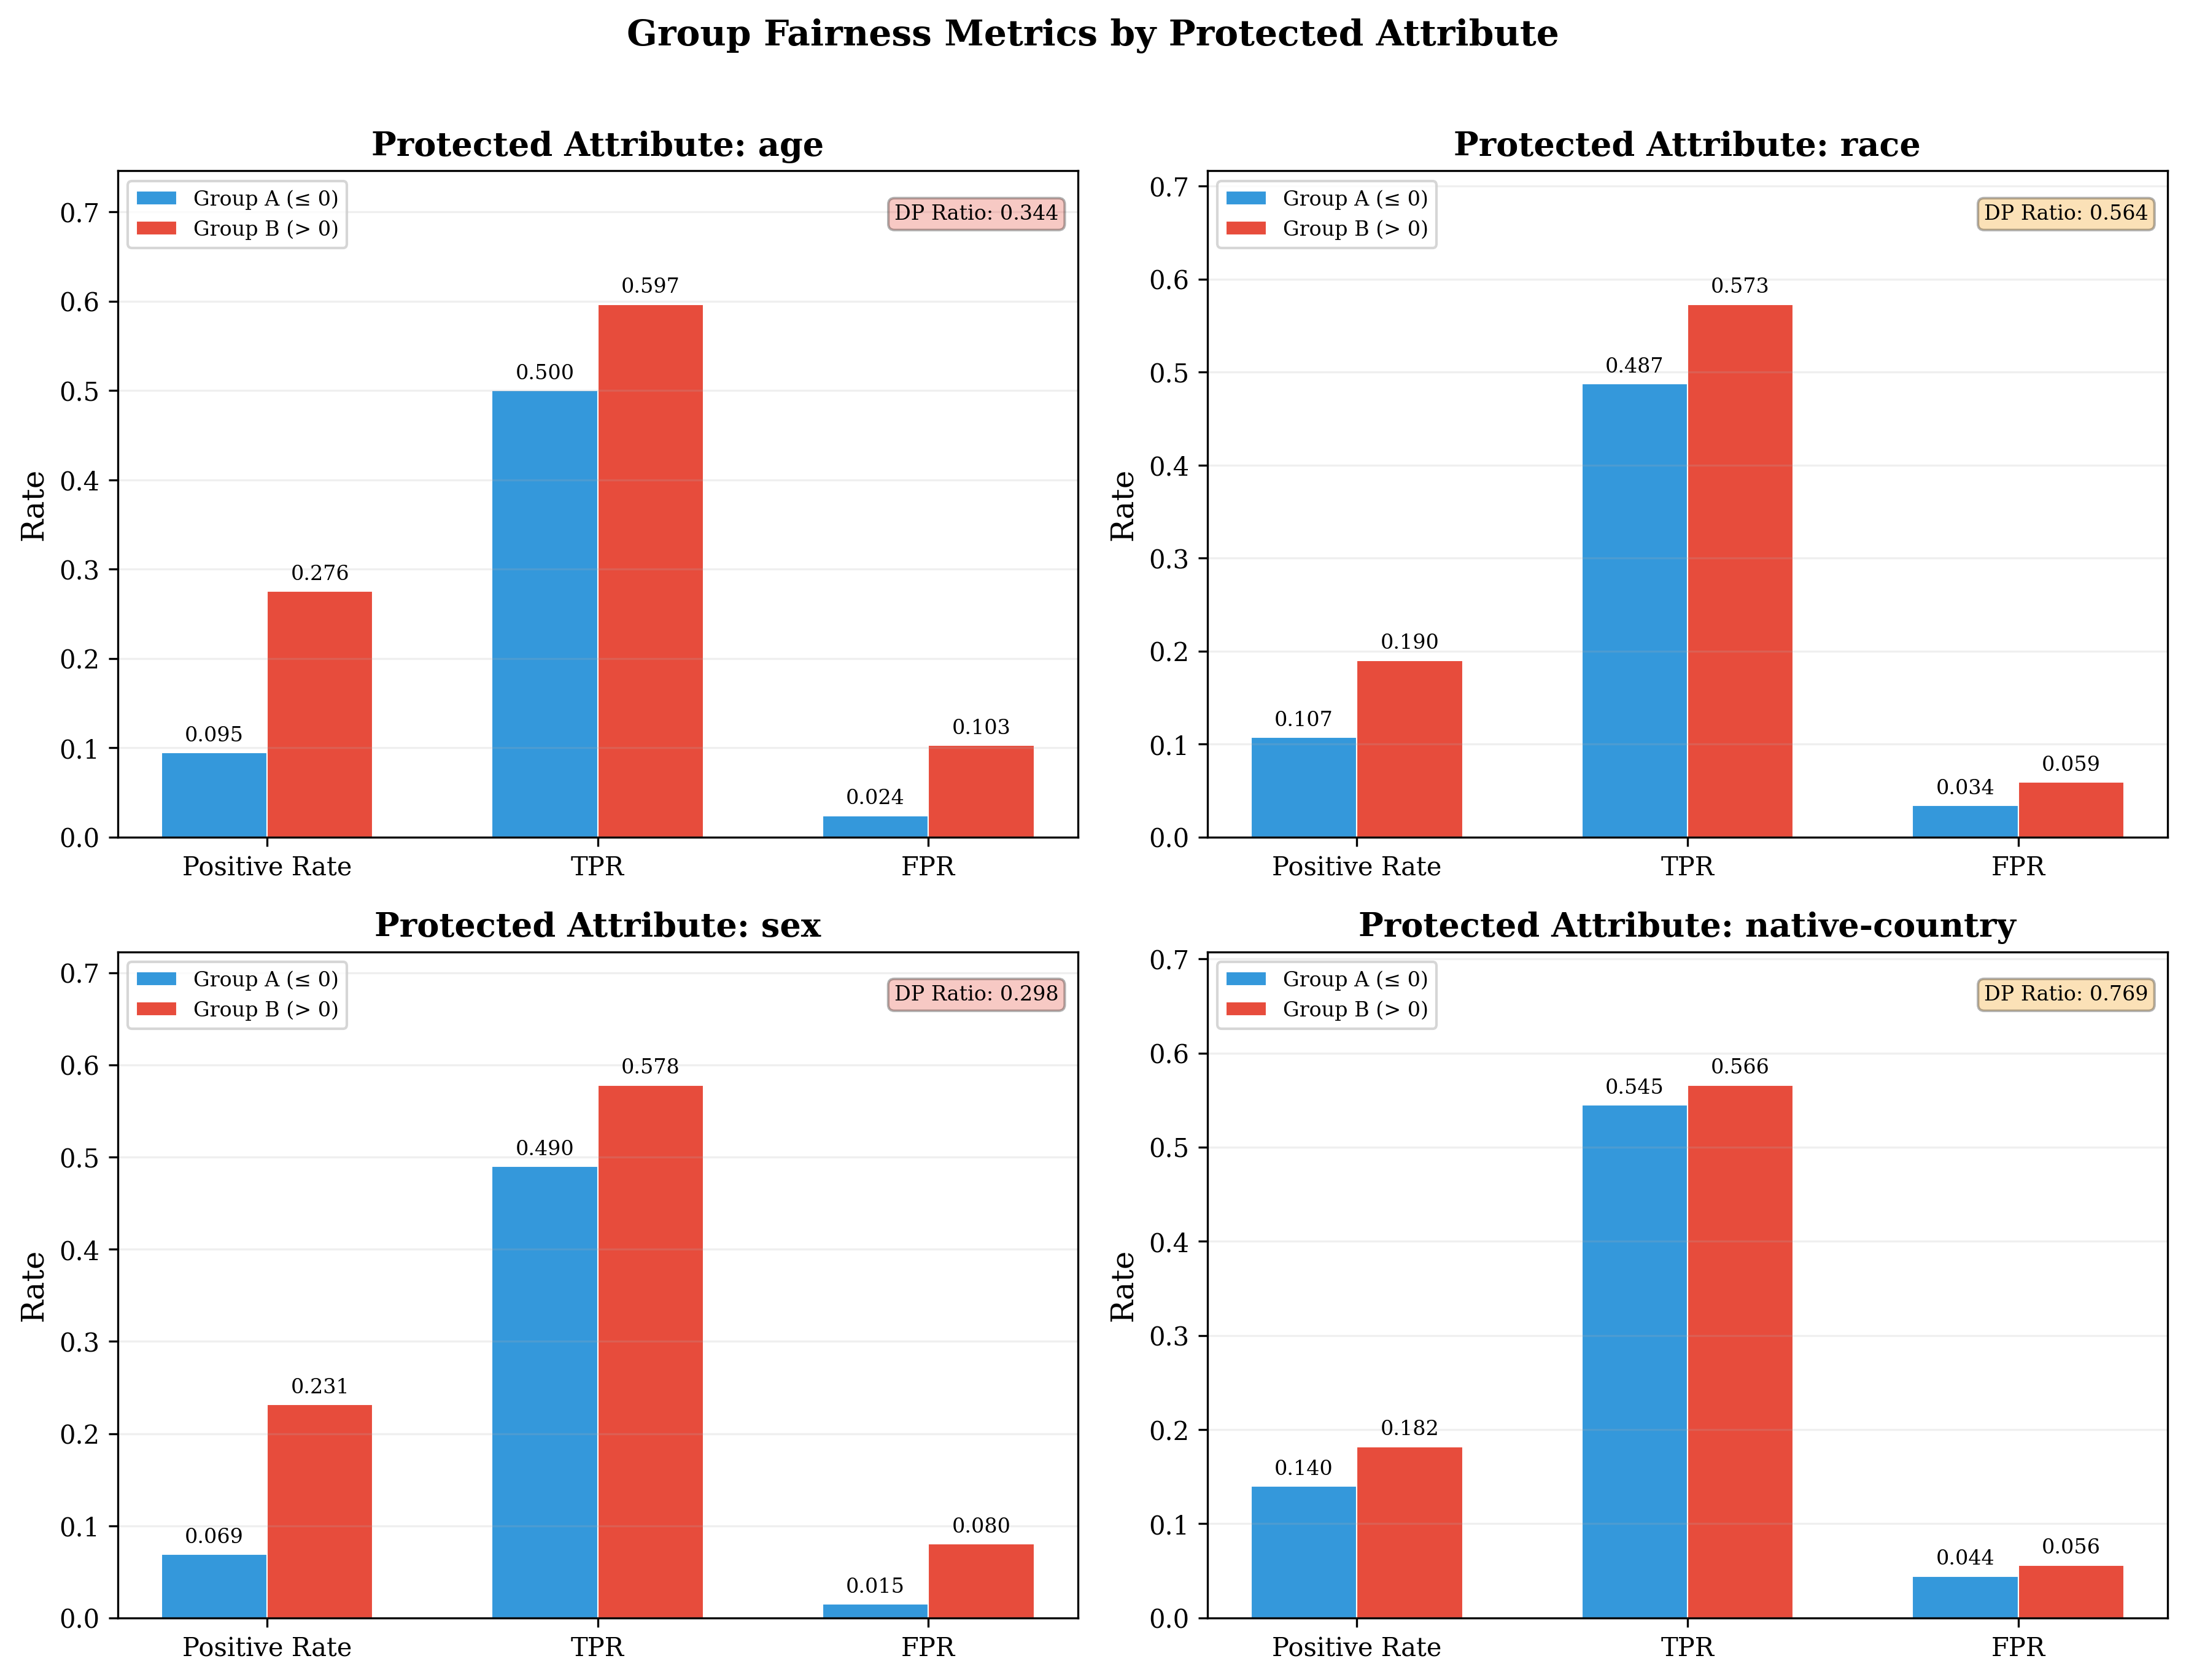
\includegraphics[width=0.95\textwidth]{images/group-fairness.png}
    \caption{Group fairness metric comparisons across protected attributes.}
    \label{fig:group_fairness}
\end{figure}

\section{Discriminatory Instance Search Results}

The gradient-guided search discovered 30 discriminatory instances. The best QID found during global search was 0.011 bits, which appears low compared to the mean QID of 0.640 bits because the search explores synthetic input regions rather than natural data instances---the search finds the input configuration where the model's counterfactual predictions are most extreme.

\section{Causal Debugging Results}

\subsection{Layer Sensitivity Analysis}

Table~\ref{tab:layer_sensitivity} presents the layer-by-layer sensitivity scores.

\begin{table}[H]
\centering
\caption{Layer sensitivity analysis results.}
\label{tab:layer_sensitivity}
\begin{tabular}{@{}lccc@{}}
\toprule
\textbf{Layer} & \textbf{Neurons} & \textbf{Sensitivity} & \textbf{Relative} \\
\midrule
Layer 1 & 64 & 1.443 & 74.7\% \\
\textbf{Layer 2} & \textbf{32} & \textbf{1.933} & \textbf{100.0\%} \\
Layer 3 & 16 & 0.769 & 39.8\% \\
Layer 4 & 8 & 0.191 & 9.9\% \\
Layer 5 & 4 & 0.188 & 9.7\% \\
Layer 6 (Output) & 2 & 0.124 & 6.4\% \\
\bottomrule
\end{tabular}
\end{table}

\textbf{Layer 2} (32 neurons) is identified as the most bias-sensitive layer with a sensitivity score of 1.933, indicating that this layer amplifies protected attribute information most strongly. Bias concentrated in early-to-middle layers suggests the network encodes protected information during initial feature transformation before it propagates through deeper layers. This finding is consistent with the causal debugging results reported by DICE~\cite{dice} on the same Adult Census dataset, which similarly identified the second layer as the most bias-sensitive.

\begin{figure}[H]
    \centering
    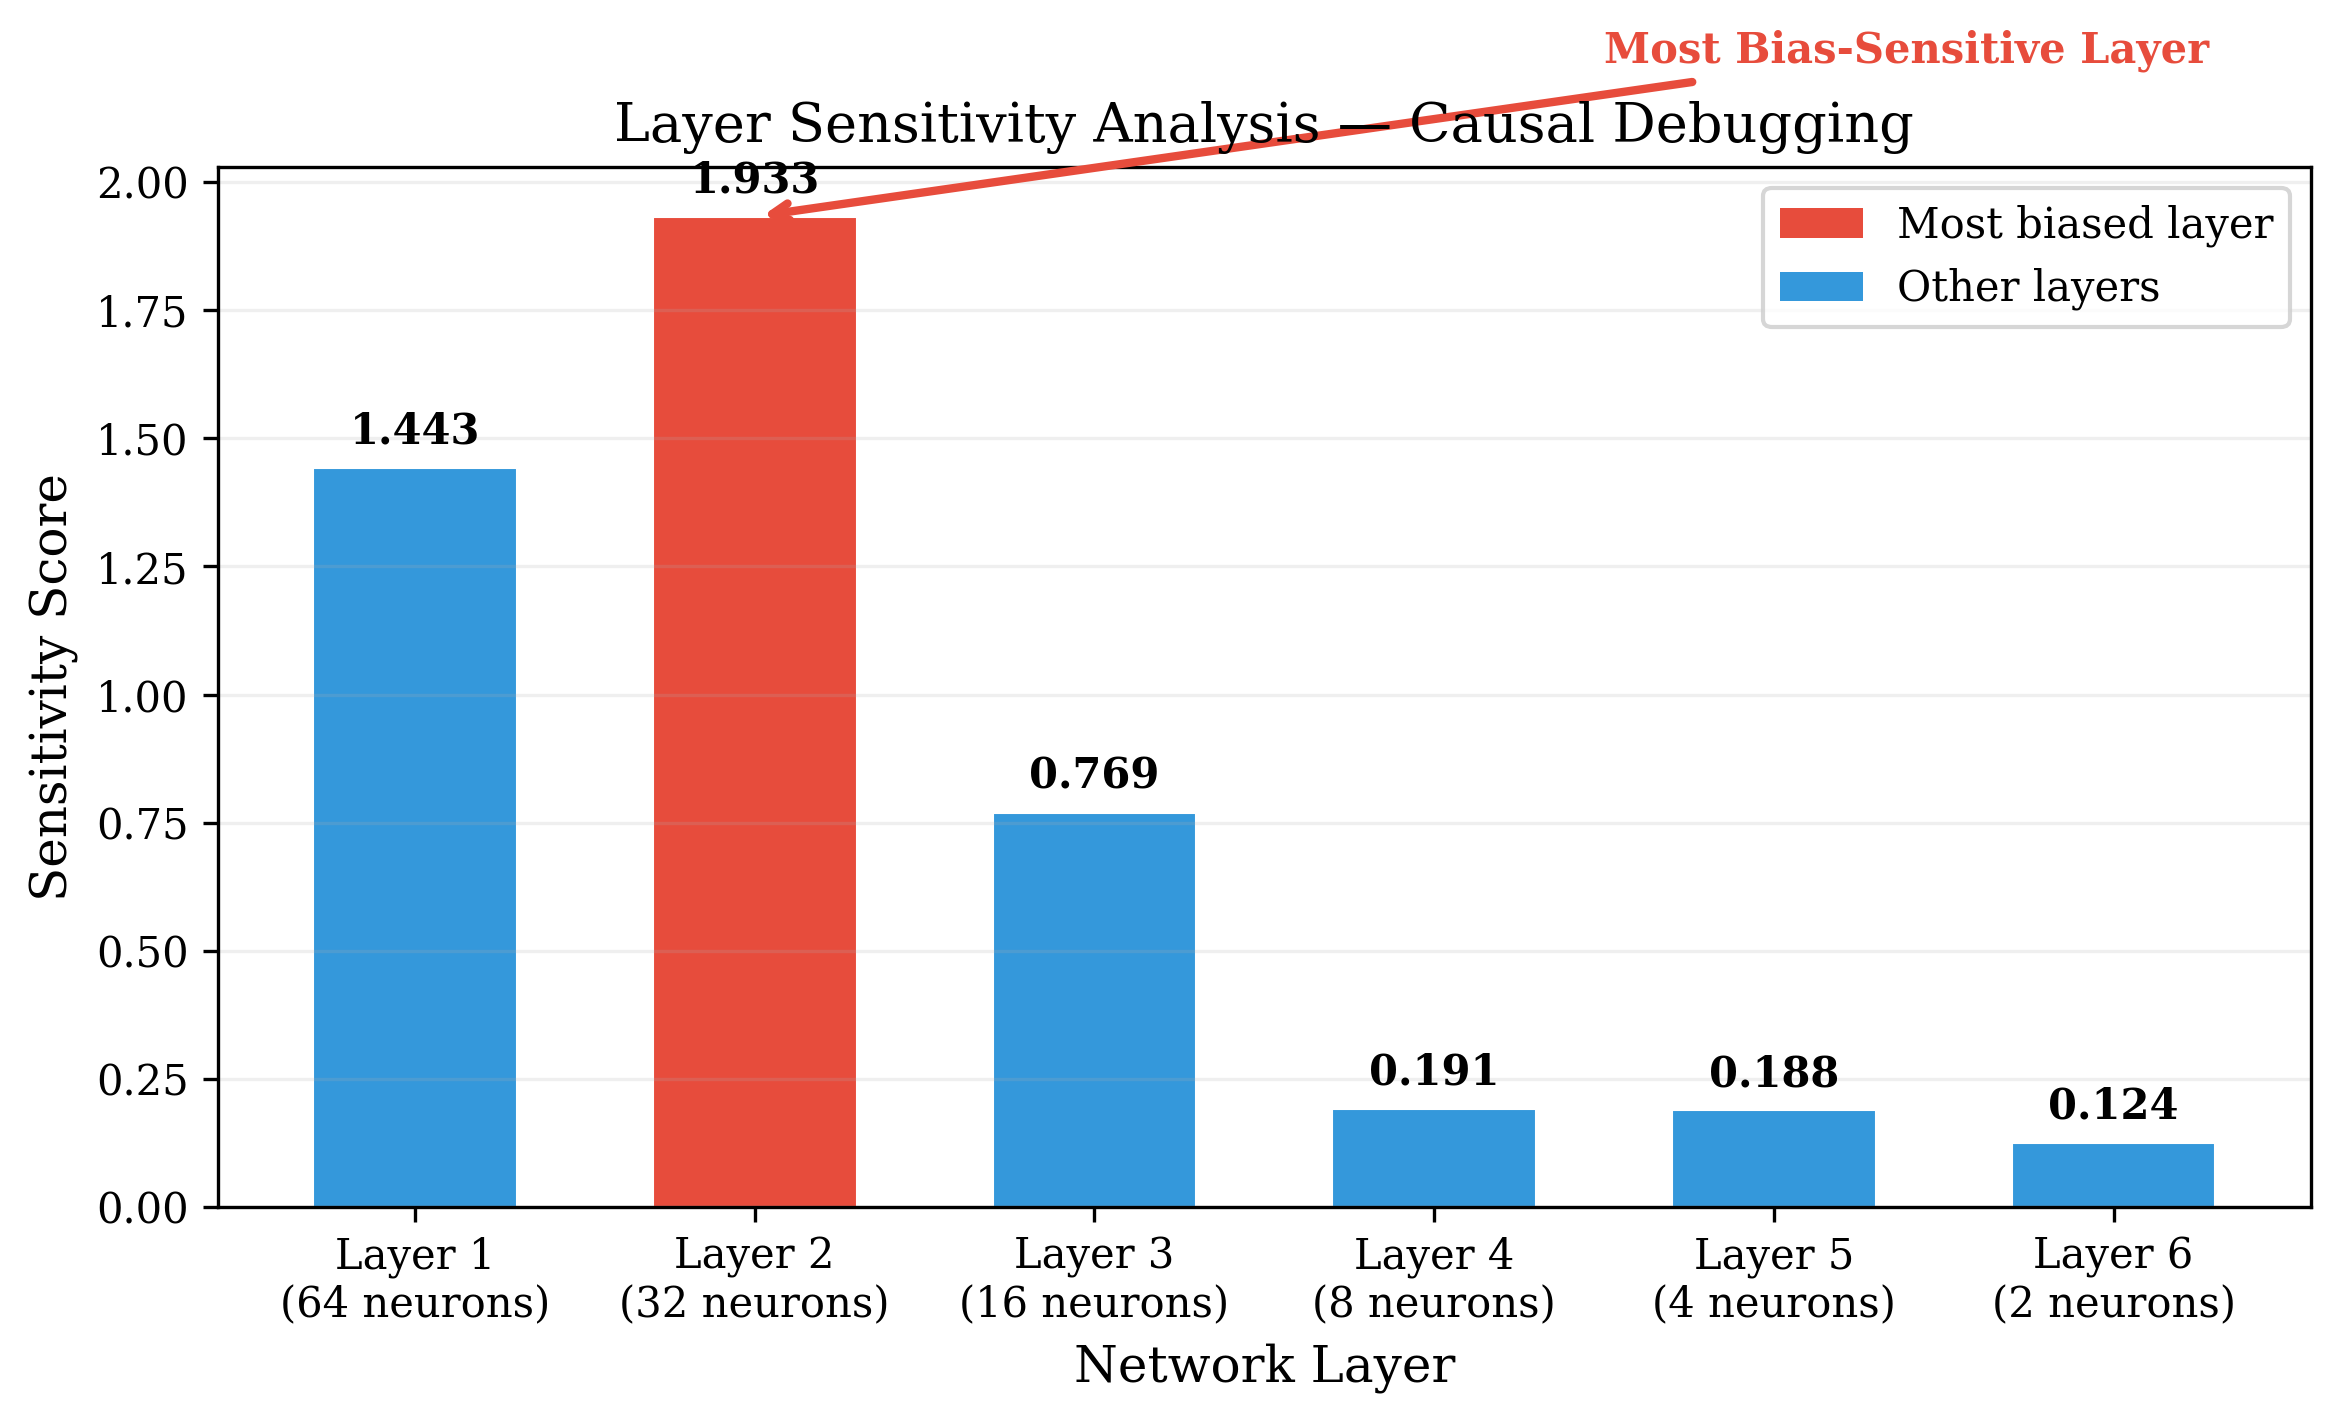
\includegraphics[width=0.95\textwidth]{images/layer-sensitivity.png}
    \caption{Layer sensitivity analysis identifying Layer 2 as the bias-critical layer.}
    \label{fig:layer_sensitivity}
\end{figure}

\subsection{Neuron-Level Analysis}

Within Layer~2, the top 5 biased neurons are:

\begin{table}[H]
\centering
\caption{Top 5 biased neurons in Layer 2.}
\label{tab:neurons}
\begin{tabular}{@{}lcc@{}}
\toprule
\textbf{Neuron} & \textbf{Impact Score} & \textbf{Relative} \\
\midrule
Neuron 30 & 1.362 & 100.0\% \\
Neuron 17 & 1.270 & 93.3\% \\
Neuron 8 & 1.220 & 89.6\% \\
Neuron 29 & 1.055 & 77.5\% \\
Neuron 23 & 0.985 & 72.3\% \\
\bottomrule
\end{tabular}
\end{table}

Neurons 30 and 17 have disproportionately high impact scores, suggesting they have specialized in encoding protected attribute information. In a fairness remediation workflow, these neurons would be primary candidates for neuron-level dropout interventions as proposed by NeuFair~\cite{neufair}.

\begin{figure}[H]
    \centering
    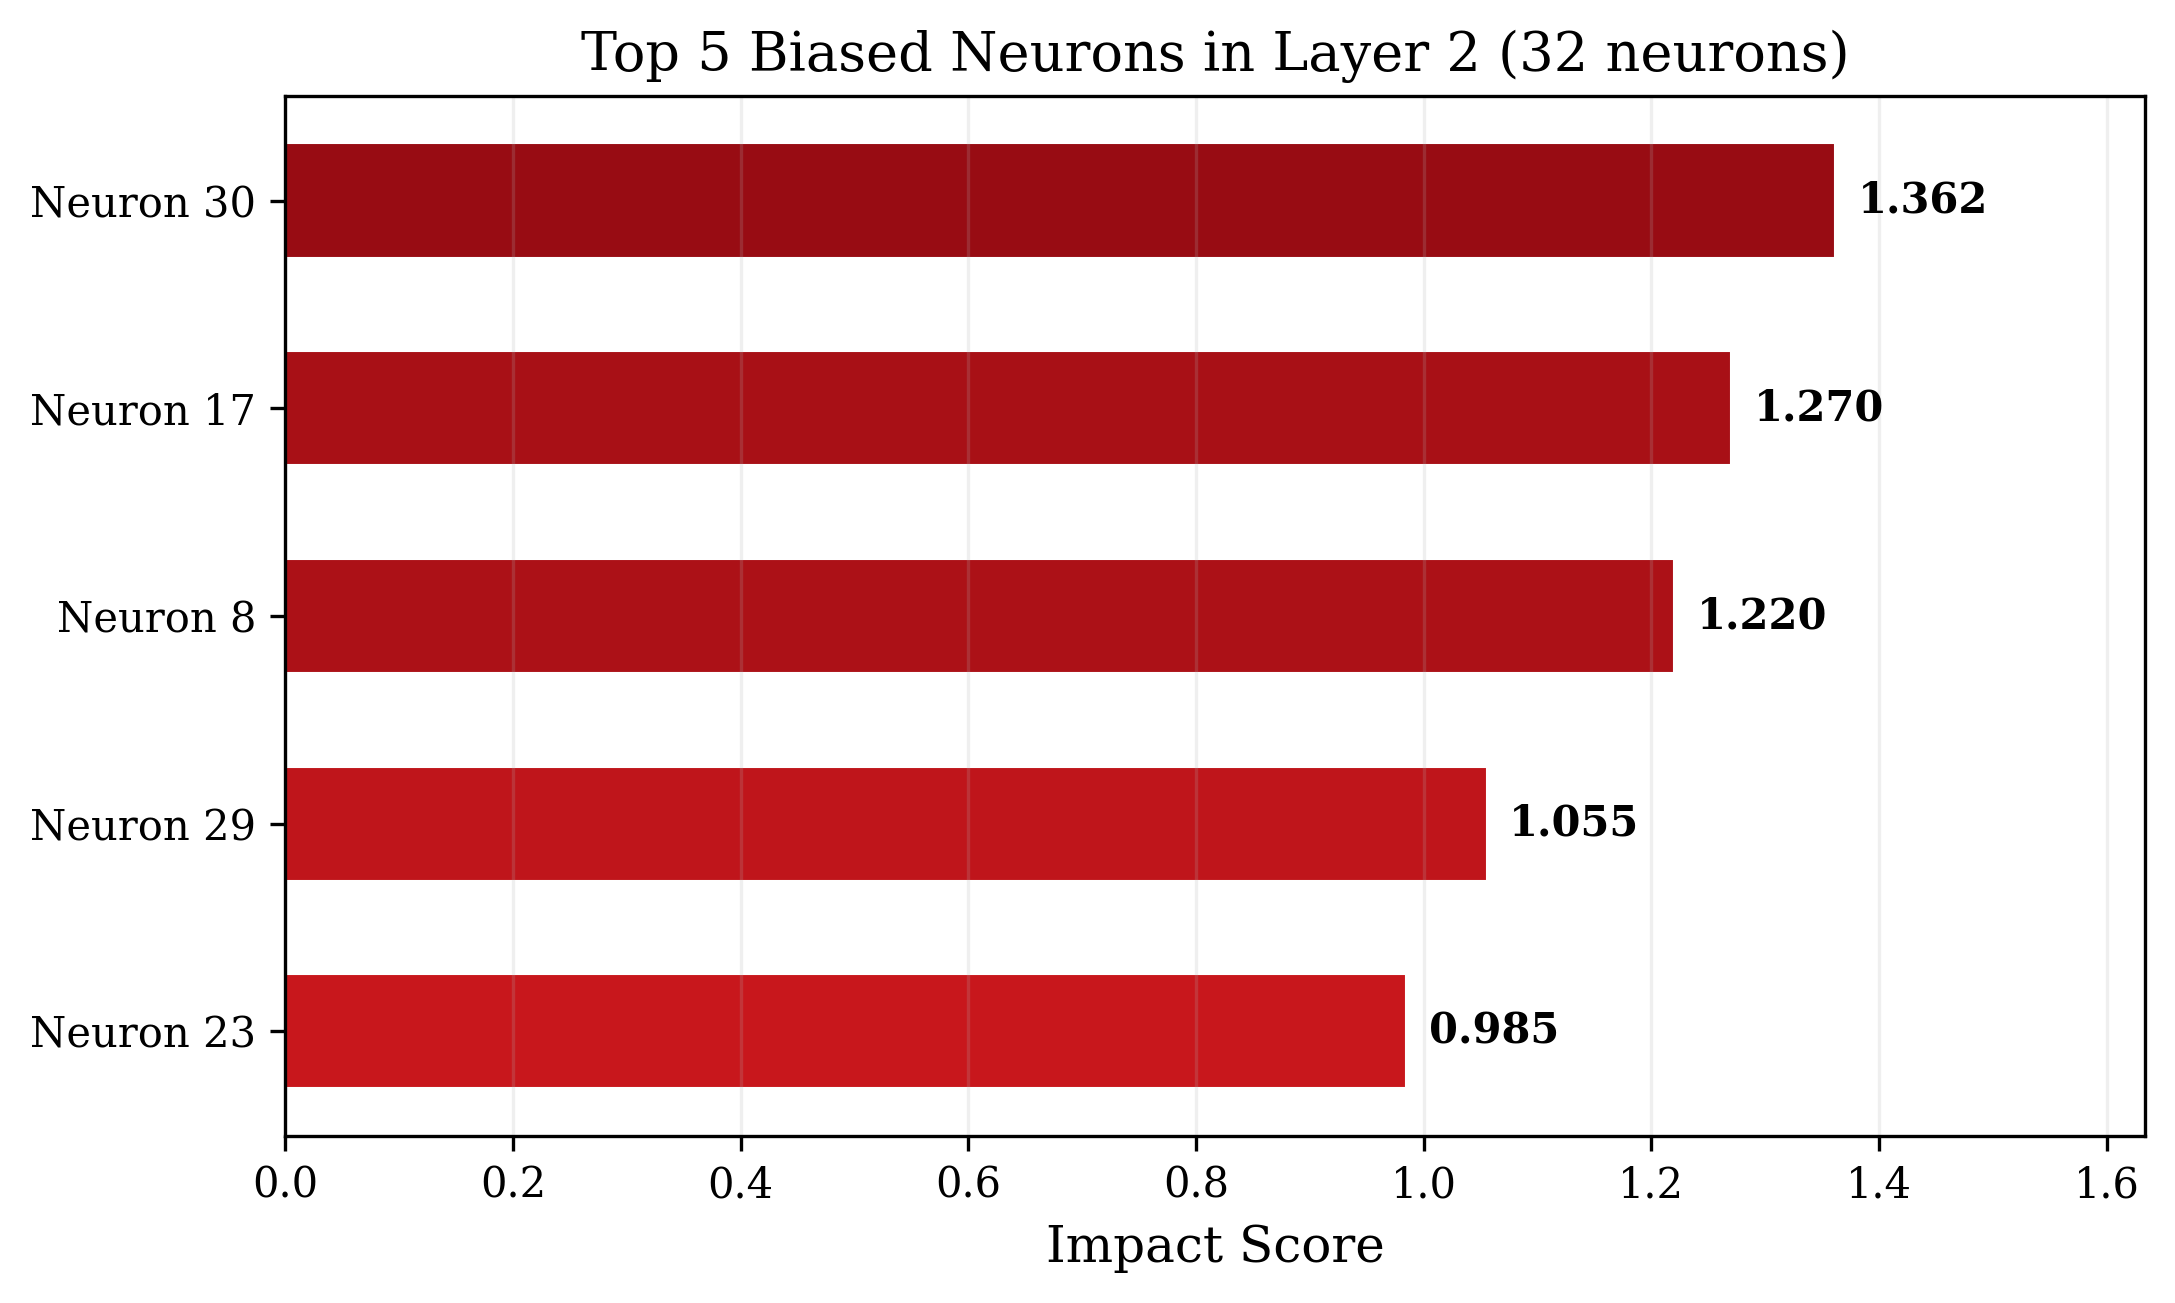
\includegraphics[width=0.95\textwidth]{images/neuron-impact.png}
    \caption{Neuron-level impact scores within Layer 2.}
    \label{fig:neuron_impact}
\end{figure}

\section{Explainability Results}

\subsection{SHAP Global Feature Importance}

Table~\ref{tab:shap} presents the SHAP global feature importance values computed on the log-odds output space.

\begin{table}[H]
\centering
\caption{SHAP global feature importance (log-odds space).}
\label{tab:shap}
\begin{tabular}{@{}clc@{}}
\toprule
\textbf{Rank} & \textbf{Feature} & \textbf{Importance} \\
\midrule
1 & education-num & 0.891 \\
2 & age$^\dagger$ & 0.690 \\
3 & marital-status & 0.688 \\
4 & hours-per-week & 0.541 \\
5 & capital-gain & 0.326 \\
6 & capital-loss & 0.233 \\
7 & relationship & 0.251 \\
8 & sex$^\dagger$ & 0.176 \\
9 & occupation & 0.115 \\
10 & education & 0.108 \\
\bottomrule
\multicolumn{3}{@{}l}{\footnotesize $^\dagger$ Protected attribute.}
\end{tabular}
\end{table}

Notably, \textbf{age} (a protected attribute) ranks \#2 in global importance, confirming that the model heavily relies on age information for predictions. \textbf{Sex} ranks \#8, indicating moderate but measurable influence. \textbf{Race} (importance: 0.010) and \textbf{native-country} (importance: 0.000) show minimal direct SHAP influence, though this does not preclude indirect influence through correlated proxy features.

\subsection{LIME Aggregated Feature Importance}

\begin{table}[H]
\centering
\caption{LIME aggregated feature importance (top 5).}
\label{tab:lime}
\begin{tabular}{@{}clc@{}}
\toprule
\textbf{Rank} & \textbf{Feature} & \textbf{Importance} \\
\midrule
1 & capital-gain & 0.246 \\
2 & education-num & 0.232 \\
3 & marital-status & 0.159 \\
4 & capital-loss & 0.156 \\
5 & hours-per-week & 0.128 \\
\bottomrule
\end{tabular}
\end{table}

Both SHAP and LIME agree that \textbf{education-num} is among the most important features, and both identify \textbf{age} as a significant protected attribute with measurable influence. This cross-method agreement provides high confidence in the feature attribution findings.

\begin{figure}[H]
    \centering
    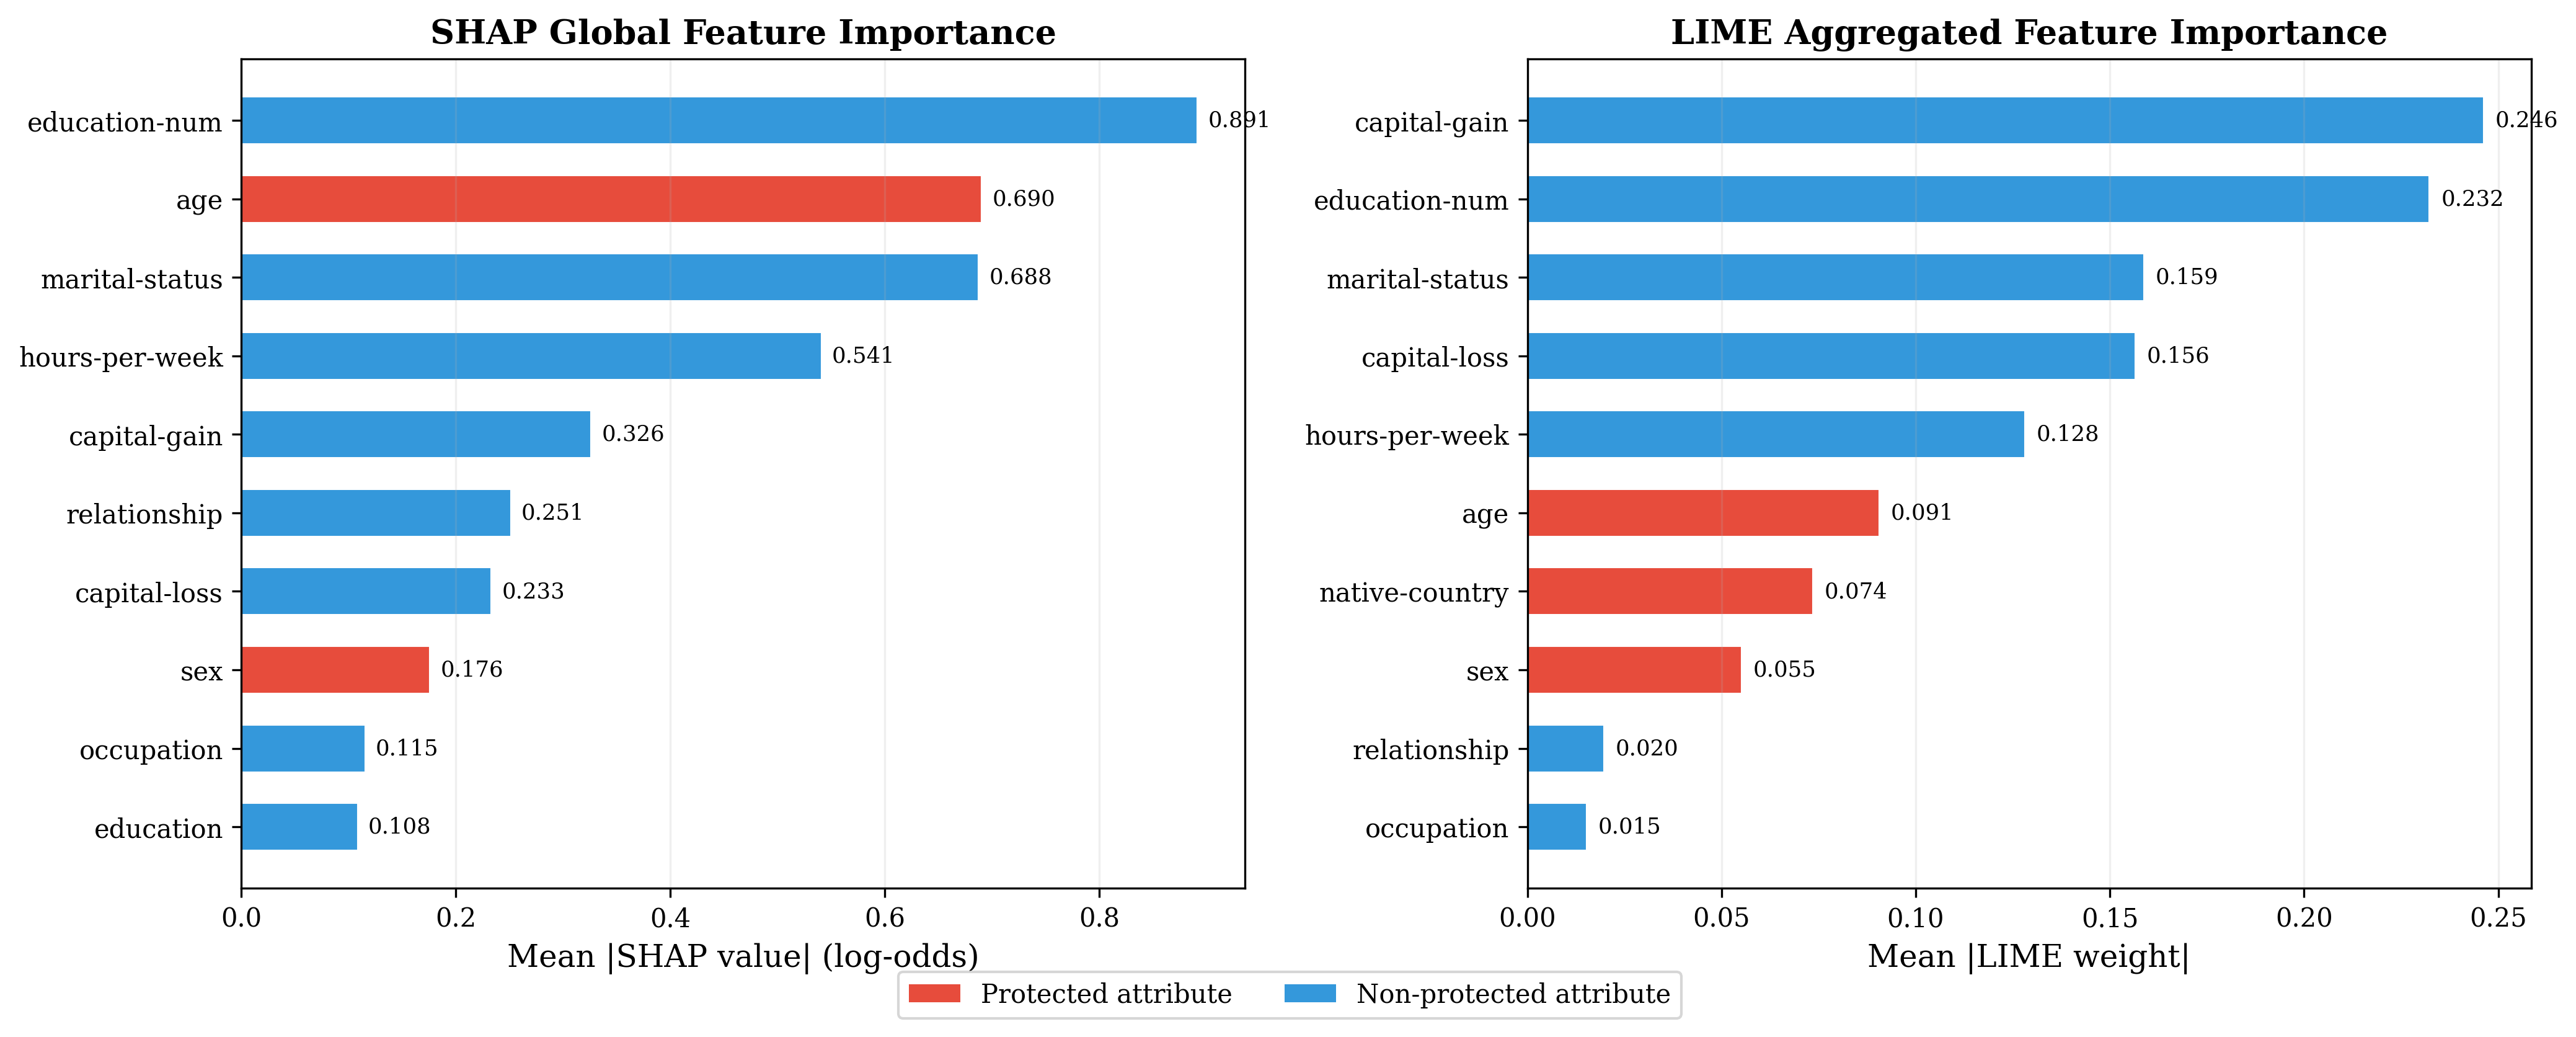
\includegraphics[width=0.95\textwidth]{images/shap-lime.png}
    \caption{SHAP and LIME feature importance comparison.}
    \label{fig:explainability}
\end{figure}

\section{Composite Fairness Score}

Applying the scoring formula from Equation~\ref{eq:score}:

\begin{table}[H]
\centering
\caption{Composite fairness score breakdown.}
\label{tab:score}
\begin{tabular}{@{}lrrr@{}}
\toprule
\textbf{Component} & \textbf{Value} & \textbf{Calculation} & \textbf{Penalty} \\
\midrule
Mean QID & 0.640 bits & $0.640 \times 15 = 9.60$ & $-10$ \\
\% Discriminatory & 95.8\% & $95.8 \times 0.3 = 28.74$ & $-29$ \\
Disparate Impact & 0.581 & $(0.8 - 0.581) \times 50 = 10.95$ & $-11$ \\
Max QID & 1.000 bits & $1.0 \times 5 = 5.0$ & $-5$ \\
Group Fairness & averaged & $(\bar{\text{DP}} + \bar{\text{EO}}) \times 25$ & $\sim$$-5$ \\
\midrule
\textbf{Total Score} & & $100 - 10 - 29 - 11 - 5 - 5$ & $\approx \mathbf{41}$ \\
\bottomrule
\end{tabular}
\end{table}

The final score of approximately \textbf{41 out of 100} is rated \textbf{``Concerning''} (red), indicating significant bias that would require substantial remediation before deployment.

\begin{figure}[H]
    \centering
    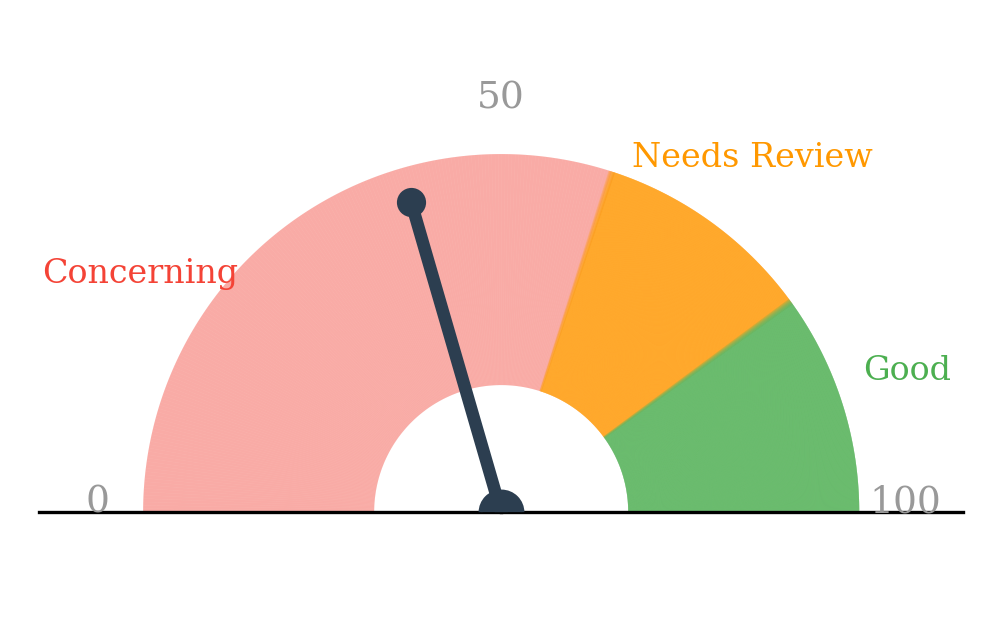
\includegraphics[width=0.95\textwidth]{images/fairness-gauge.png}
    \caption{Composite fairness score gauge for the Adult Census dataset.}
    \label{fig:gauge}
\end{figure}

\section{Performance Timing}

\begin{table}[H]
\centering
\caption{Analysis pipeline timing (cached model).}
\label{tab:timing}
\begin{tabular}{@{}lr@{}}
\toprule
\textbf{Step} & \textbf{Duration (s)} \\
\midrule
Model Training (cached) & 1 \\
Activations & 1 \\
QID Analysis + Group Fairness & 1 \\
Discriminatory Instance Search & 2 \\
Causal Debugging & $<$1 \\
SHAP + LIME Explanations & 7 \\
\midrule
\textbf{Total} & \textbf{12} \\
\bottomrule
\end{tabular}
\end{table}

With model caching, the full analysis completes in approximately 12 seconds, demonstrating the feasibility of integrating comprehensive fairness analysis into the developer workflow. First-run training adds approximately 77 seconds for the Adult Census dataset.
